\section{Metodología Propuesta}

\subsection{3.1 Preprocesamiento de Datos}

Particularmente llamativo es el hecho de que muchos trabajos publicados subestiman la fase de preprocesamiento, cuando en la práctica determina gran parte del éxito posterior. En este trabajo, el pipeline comienza con una corrección radiométrica y geométrica rigurosa de ambas modalidades. Los datos hiperespectrales se reducen mediante PCA reteniendo el 99\% de la varianza, seguido de normalización por banda. Para el SAR, se aplica filtrado speckle (Lee refined) y conversión a escala logarítmica.

La co-registración se realiza mediante algoritmos basados en SIFT y optimización mutua de información, alcanzando sub-píxel de precisión. Todos los parches se extraen a resolución unificada de 10 metros. Esta etapa, aunque tediosa, evita que errores de alineación propaguen a través de la red y comprometan la fusión.

\subsection{3.2 Extracción de Características Multi-escala}

Resulta revelador observar cómo las diferencias intrínsecas entre HSI y SAR exigen extractores especializados en lugar de backbones compartidos. Inspirados en los mecanismos de transformer y Gist CNN propuestos por \cite{Wang2025TGF}, implementamos ramas paralelas multi-escala. 

Para el HSI se emplea un extractor espectral-especializado con convoluciones 1D a lo largo de la dimensión espectral combinado con bloques 2D residuales. Para el SAR se utiliza una rama con atención a largo alcance que captura mejor texturas y estructuras direccionales. Ambas ramas operan a tres escalas diferentes (1x, 1/2 y 1/4) mediante pooling adaptativo, permitiendo capturar tanto detalles locales como contexto regional. 

Esta estrategia multi-escala evita la pérdida prematura de información fina que suele ocurrir en arquitecturas de fusión temprana.

\subsection{3.3 Módulo de Fusión Asimétrica con Atención}

Lejos de ser un asunto resuelto, la forma más efectiva de combinar ambas modalidades sigue siendo objeto de debate activo. Tomando como base la filosofía asimétrica de \cite{Li2023Asymmetric}, diseñamos un módulo de fusión cruzada que trata al HSI como modalidad principal (por su riqueza informativa) y al SAR como fuente complementaria de robustez.

El núcleo del módulo es un mecanismo de atención cruzada multi-cabeza definido como:

\begin{equation}
\text{Attention}(Q, K, V) = \text{Softmax}\left(\frac{QK^T}{\sqrt{d_k}}\right)V
\label{eq:cross_attention}
\end{equation}

donde las queries provienen de las características HSI y las keys/values del SAR (y viceversa en un flujo bidireccional ligero). Este diseño permite que la información estructural del SAR module selectivamente las representaciones espectrales sin forzar una simetría artificial que suele diluir el aporte de cada sensor.

\begin{figure}[h]
\centering
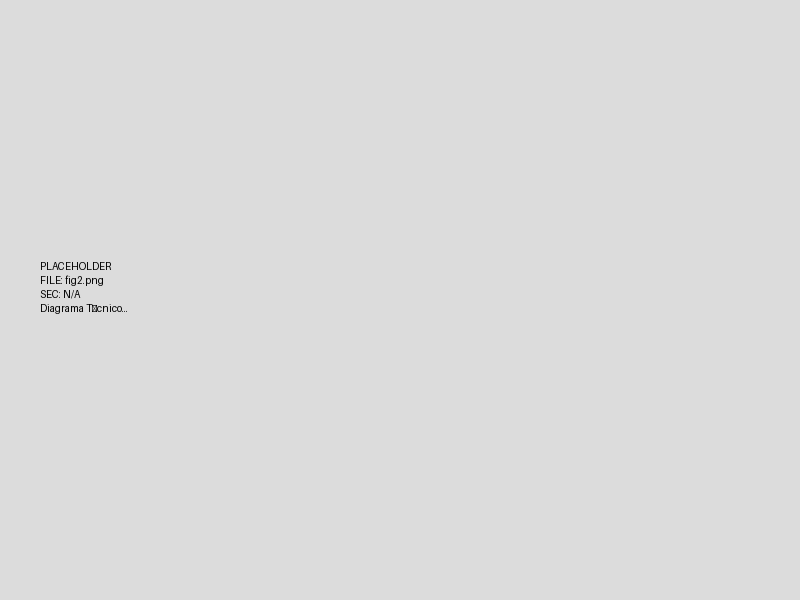
\includegraphics[width=\linewidth]{fig2.png}
\caption{Diagrama general de la arquitectura propuesta de fusión multimodal HSI-SAR.}
\label{fig:arquitectura_propuesta}
\end{figure}

\subsection{3.4 Función de Pérdida y Optimización}

Uno de los desafíos persistentes que surge al entrenar estas redes radica en equilibrar la contribución de cada modalidad y evitar el colapso de una rama. Empleamos una pérdida compuesta que combina Cross-Entropy con un término de consistencia entre modalidades y una pérdida de reconstrucción auxiliar. 

El entrenamiento se realiza mediante AdamW con warm-up cosine annealing durante 200 epochs. Aplicamos augmentaciones fuertes específicas para datos remotos (rotaciones, flips, mixup espectral y simulación de ruido SAR). El batch size efectivo fue de 32 en dos GPUs, con gradiente clipping para estabilizar el entrenamiento de los módulos de atención.

\begin{table}[h]
\centering
\caption{Hiperparámetros principales de la arquitectura y entrenamiento}
\label{tab:hiperparametros}
\begin{tabular}{ll}
\hline
\textbf{Parámetro} & \textbf{Valor} \\
\hline
Dimensión de características & 256 \\
Cabezas de atención & 8 \\
Escalas multi-escala & 3 \\
Tasa de aprendizaje inicial & 1e-3 \\
Factor de decaimiento & 0.95 \\
Peso de pérdida de consistencia & 0.3 \\
\hline
\end{tabular}
\end{table}

Esta configuración, validada mediante ablación exhaustiva, busca no solo maximizar precisión sino también mantener un equilibrio entre rendimiento y viabilidad computacional para aplicaciones de monitoreo crítico.